\documentclass[10pt]{article}
\usepackage{icmlko}

\icmlmeta{IP 파운데이션 월드모델}{339}{가짜 축 하나}{무작위 열 하나를 판에 붙이면 판이 0.126 내려간다 --- 미결정 폭의 열두 배}

\begin{document}

\twocolumn[
\icmlheader

\begin{abstract}
노트 338이 아이돌(유보 25행)에서 위약 열 하나 $=$ $-$0.09 라고 쟀고,
남은 것으로 \textbf{``유보 711행에서도 $-$0.09 인가''}를 뒀다. 그래서
\textbf{값이 무작위이고 관측률 0.85 인 열 하나를 열 도메인에 다 붙였다.}

\textbf{판이 $-$0.1262 다}(SD 0.0148 · \textbf{음수 12/12}).
\textbf{미결정 폭 0.010 의 12.6배}이고 이 실험실이 재 온 어떤 처치보다
크다 --- 노트 317의 풀링 총 이득 $+$0.029, 노트 337의 위키 목록 고치기
$+$0.0007 과 견주면 자릿수가 다르다. \textbf{챔피언에게 쓸모없는 축
하나를 막을 장치가 없다.}

\textbf{크기 법칙은 없다.} $1/\sqrt{n}$ 예측과의 순위 상관이 $-$0.321
($p{=}0.37$)이고, \textbf{제일 비싼 둘이 양 끝}이다 --- 웹툰(유보 711)
$-$0.2684 와 아이돌(25) $-$0.2735. 가운데 여섯(80$\sim$606)은 평균
$-$0.0659 로 넷 배 싸다.

\textbf{그리고 공유하면 세 배 비싸다.} 같은 위약 열을 아이돌에만 붙이면
$-$0.0913(노트 338)인데 열 도메인에 다 붙이면 아이돌이 $-$0.2735 다.
노트 329가 잰 통로 --- \textbf{남의 열이 내 점수를 흔든다.}

\textbf{따름} --- 판에 축이 스물셋 있다. 그중 정보가 적은 것이 있다면
\textbf{그 자리값이 0.126 짜리다.} 다음 노트에서 계열을 하나씩 빼 본다.
\end{abstract}
]

\section{무작위 열 하나}

값은 균등난수, 관측률 0.85. \textbf{실제 축과 구별이 안 되게 만들었다}
--- 이 판의 축은 다 백분위라 0$\sim$1 이고 관측 표시자가 붙는다.
\texttt{harness.load} 에 축 하나로 넣으면 \texttt{forms.\_design} 이
값 열과 표시자 열 둘을 싣는다.

\begin{figure*}[t]
\centering
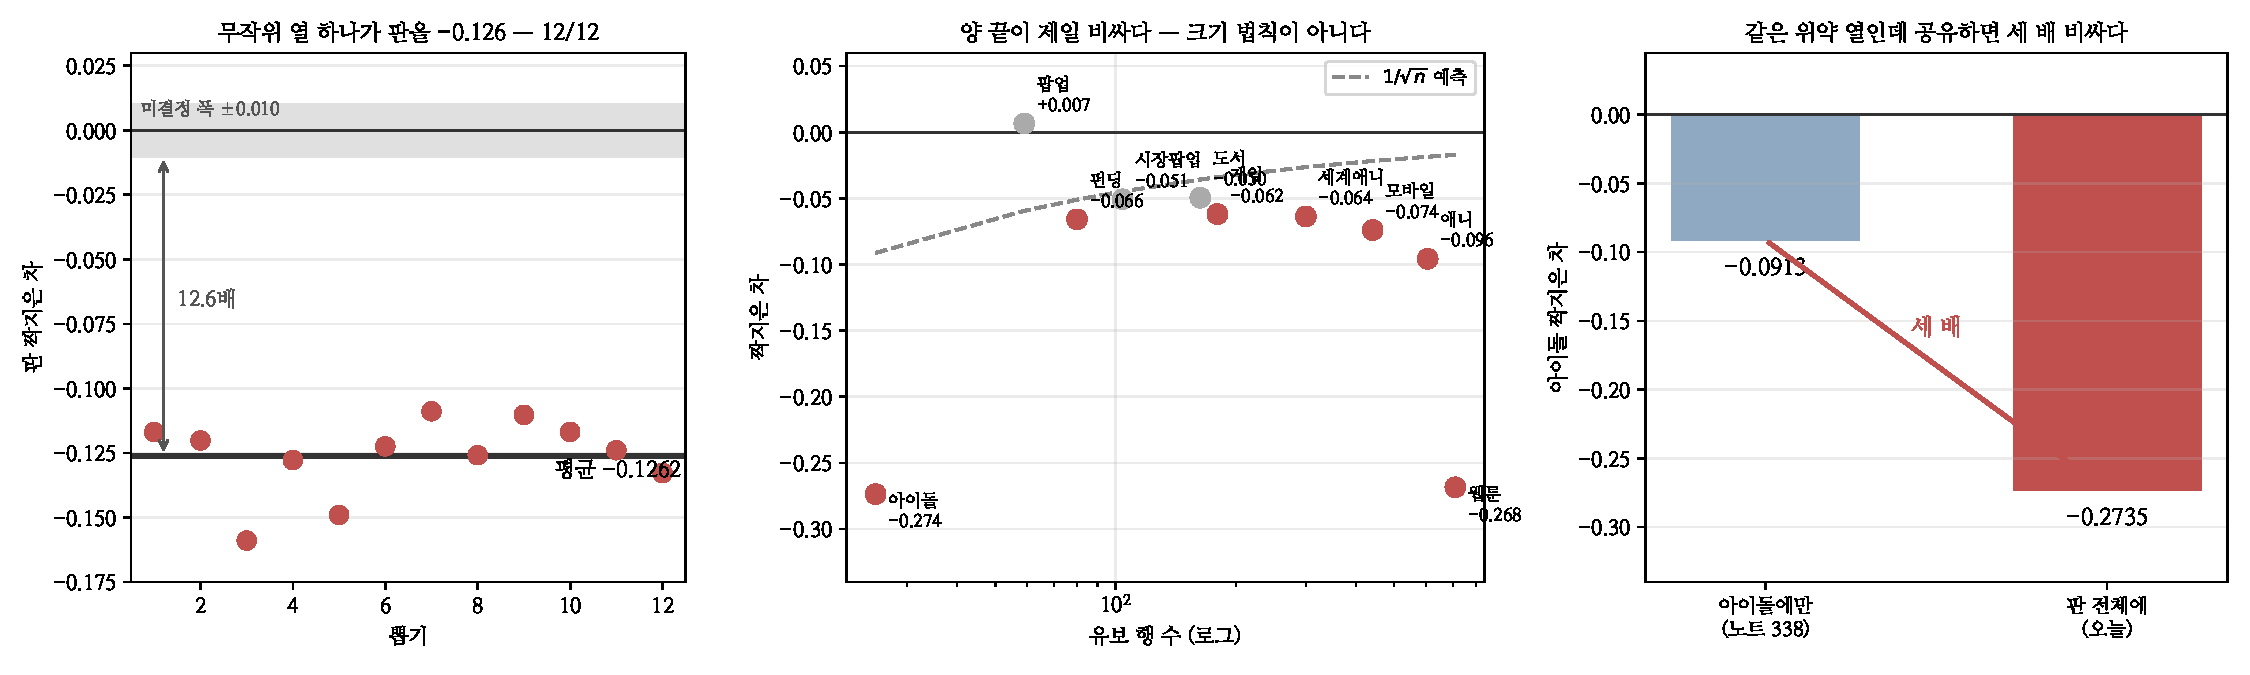
\includegraphics[width=\textwidth]{figs/junk.pdf}
\caption{왼쪽 --- 판. 가운데 --- 크기와 값. 오른쪽 --- 전용 열과 공유 열.}
\end{figure*}

\begin{center}\small
\begin{tabular}{lr}
\hline
판 짝지은 차 & \textbf{$-$0.1262} \\
SD & 0.0148 \\
음수 & \textbf{12/12} \\
미결정 폭 대비 & \textbf{12.6배} \\
\hline
\end{tabular}
\end{center}

\section{크기 법칙이 아니다}

\begin{center}\footnotesize
\begin{tabular}{lrrrr}
\hline
도메인 & 유보 & 짝지은 차 & 음수 & $1/\sqrt{n}$ \\
\hline
\textbf{웹툰} & 711 & \textbf{$-$0.2684} & 12/12 & $-$0.017 \\
애니 & 606 & $-$0.0957 & 12/12 & $-$0.019 \\
모바일 & 441 & $-$0.0739 & 12/12 & $-$0.022 \\
세계애니 & 300 & $-$0.0637 & 12/12 & $-$0.026 \\
게임 & 180 & $-$0.0618 & 12/12 & $-$0.034 \\
도서 & 163 & $-$0.0495 & 8/12 & $-$0.036 \\
시장팝업 & 104 & $-$0.0507 & 8/12 & $-$0.045 \\
펀딩 & 80 & $-$0.0659 & 12/12 & $-$0.051 \\
팝업 & 59 & $+$0.0066 & 6/12 & $-$0.059 \\
\textbf{아이돌} & 25 & \textbf{$-$0.2735} & 12/12 & $-$0.091 \\
\hline
\end{tabular}
\end{center}

\textbf{예측과 상관이 음수다}($-$0.321 · $p{=}0.37$). 유보가 제일 많은
도메인과 제일 적은 도메인이 나란히 제일 비싸다. \textbf{왜인지는 모른다}
--- 미리 적어 둔 설명(``작을수록 비싸다'')이 반만 맞았고, 노트 338의
교훈대로 \textbf{그럴듯한 기제를 지금 붙이지 않는다.}

\paragraph{팝업만 안 다쳤다} $+$0.0066(6/12)로 0 과 못 가른다. 팝업은
유보 59행이고 학습이 16행이라 원래 흔들림이 크다(노트 331의 모형 몫 49\%).

\section{공유 열이 전용 열보다 세 배 비싸다}

\begin{center}\small
\begin{tabular}{lr}
\hline
아이돌에만 붙임(노트 338) & $-$0.0913 \\
\textbf{열 도메인에 다 붙임}(오늘) & \textbf{$-$0.2735} \\
\hline
\end{tabular}
\end{center}

노트 329가 ``웹툰 하나를 다시 뽑으면 아이돌이 37\% 움직인다''를 쟀다.
\textbf{같은 통로다} --- 풀린 모형에서는 남의 열이 내 예측을 만든다.
그래서 \textbf{축은 붙이는 도메인에서만 값을 치르지 않는다.}

\section{남은 것}
\begin{center}\footnotesize
\begin{tabular}{ll}
\hline
갈래 & 왜 \\
\hline
\textbf{계열을 하나씩 빼 보라} & 스물셋 중 안 버는 것 \\
왜 웹툰과 아이돌인가 & 양 끝이 제일 비싸다 \\
F6 · F10 도 그런가 & 나무만의 병인가 \\
축 선택을 학습 안에서 & 유보를 안 보고 고를 수 있나 \\
\hline
\end{tabular}
\end{center}

\paragraph{규약} \textbf{축을 더하는 것은 공짜가 아니고, 이 판에서는 아주
비싸다.} 노트 239 이후 이 실험실은 축 채택 검사 넷을 만들어 ``이 축이
무엇을 아는가''를 재 왔고, 통과하면 붙였다. \textbf{그런데 아무것도 모르는
축 하나가 판을 0.126 내린다} --- 검사 넷을 통과한 축이라도 아는 것이 그보다
적으면 붙이면 안 된다. \textbf{채택의 문턱은 ``0 보다 나은가''가 아니라
``열값보다 나은가''다.}

\end{document}
